\documentclass[11pt, xcolor = {dvipsnames}]{beamer}
\usetheme{Malmoe}
\usepackage[utf8]{inputenc}
\usepackage[english]{babel}
\usepackage{amsmath}
\usepackage{amsfonts}
\usepackage{amssymb}
\usepackage{graphicx}
\usepackage{hyperref}

\usepackage{booktabs}
\usepackage{tabulary}
\usepackage{notes}
\usepackage{comment}
\usepackage{listings}
\usepackage{multirow}
\usepackage{adjustbox}
\usepackage{tikz}
	\usetikzlibrary{arrows.meta}
	\usetikzlibrary{arrows}
	\usetikzlibrary{shapes}
	\usetikzlibrary{fit}
\author{Julien Gori}
\title{WAI Meeting}
\subtitle{\emph{interaction-agents} \\ A Python library for Computational HCI}
%\setbeamercovered{transparent} 
%\setbeamertemplate{navigation symbols}{} 
%\logo{} 
%\institute{} 
\date{July 2021} 
%\subject{} 


\usepackage[style=authoryear,backend=bibtex]{biblatex}
\addbibresource{../paper/lib.bib}


\newcommand\blfootnote[1]{%
  \begingroup
  \renewcommand\thefootnote{}\footnote{#1}%
  \addtocounter{footnote}{-1}%
  \endgroup
}



\newcommand{\bbmf}[1]{{\textbf{\usebeamercolor[fg]{title} #1}}}
\newcommand{\bmf}[1]{{\usebeamercolor[fg]{title} #1}}


\begin{document}

\begin{frame}
\titlepage
\end{frame}




\section{Introduction}

\begin{frame}{\textbf{Computational HCI (CHCI)}}
\begin{itemize}
\item \bbmf{User-centered design} $\longrightarrow$ \textbf{best design}: iterations between designs \& empirical evaluations $=$ Costly \& highly dependent on the person conducting the design process.
\item \bbmf{Computational HCI} $\longrightarrow$ \textbf{optimal design}: minimization of some cost function to inform design $=$ Less costly (simulation-based), more objective
\end{itemize}
\end{frame}


\begin{frame}{\textbf{Ingredients of CHCI}}
\begin{enumerate}
\item \bbmf{Synthetic User Models}: describe human behavior in terms (e.g. NN, likelihood, rules) usable by an algorithm $\longrightarrow$ Sciences that study the Human e.g; (computational) cognitive scientists, behavioral scientists.
\item \bbmf{Artificial Systems} (the ``end-product''): Interface that usually exploits a user model $\longrightarrow$ various breeds of computer scientists.
	\begin{itemize}
	\item Limited standardization
	\item Often implemented in languages not destined to computational modeling
	\end{itemize}
\item \bbmf{Simulation/Evaluation}: 
	\begin{itemize}
	\item Assess whether the couple (synthetic user model, artificial system) works. 
	\item One way for artificial system to exploit user models. 
	\item Evaluate artificial systems against real users. 
	\end{itemize}
	
\end{enumerate}
\end{frame}

\begin{frame}{\textbf{CHCI is hard}}
\begin{itemize}
\item Complete system requires knowledge from many fields (user modeling, building software, learning/decision making algorithms, experimental science)
\item Low replicability / re-use of other researcher's work
	\begin{itemize}
		\item Language problem (computing language / interface language)
		\item Often full systems released, with few or no modules that can be reused by others
		\item Usually baselines have to be re-implemented.
	\end{itemize}
\item Evaluation on real interfaces rarely done
\end{itemize}

\end{frame}


\begin{frame}{\textbf{Python library: interaction-agents}}
Main idea of the library:
\begin{enumerate}
\item The interaction between a user and an artificial system can be modeled as a Partially Observable Stochastic Game (POSG)
\item The state-transition and observation function of the POSG can be decomposed into several components
\item The library provides a common interface for each component (\bmf{standardization})
\item Components can be plugged together to form higher level components (\bmf{modularity})
\end{enumerate}

\end{frame}

\section{Interaction Model}


\begin{frame}{\textbf{User-Assistant Model}}
\begin{minipage}{.6\textwidth}
\includegraphics[height = .8\textheight]{fig/two_agents_generic.pdf} 
\end{minipage}
\begin{minipage}{.38\textwidth}
\begin{itemize}
\item Users and assistants are decision making systems
\item States: task ($s_T$), user ($s_O$), assistant ($s_A$).
\end{itemize}
\end{minipage}
\end{frame}


\begin{frame}{\textbf{Sequential Decision Making}}
\resizebox{!}{.8\textheight}{
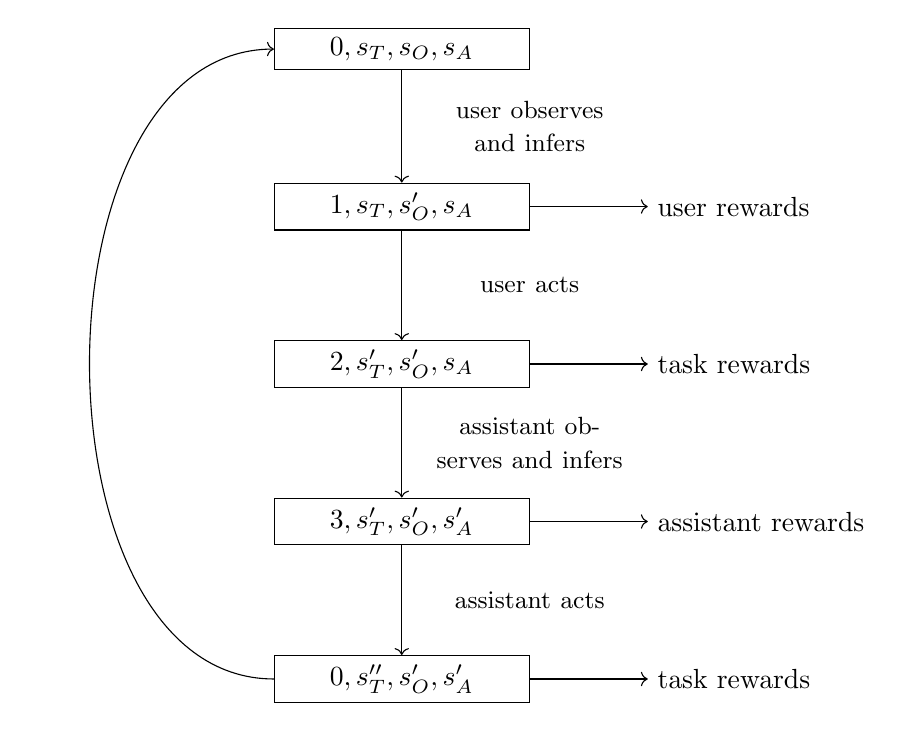
\begin{tikzpicture}
\draw (0,0) node[rectangle, draw = black, name = s0, text width = 3cm, text centered]{$0,s_T, s_O, s_A$};
\draw (s0) + (0,-2) node[rectangle, draw = black, name = s1, text width = 3cm, text centered]{$1,s_T, s'_O, s_A$};
\draw[->] (s0) -- node[midway, right, text width = 3cm, text centered]{\small user observes and infers} (s1);
\draw[->] (s1.0) -- + (1.5,0) node[right]{user rewards};
\draw (s1) + (0,-2) node[rectangle, draw = black, name = s2, text width = 3cm, text centered]{$2,s'_T, s'_O, s_A$};
\draw[->] (s1) -- node[midway, right, text width = 3cm, text centered]{\small user acts} (s2);
\draw[->] (s2.0) -- + (1.5,0) node[right]{task rewards};
\draw (s2) + (0,-2) node[rectangle, draw = black, name = s3, text width = 3cm, text centered]{$3,s'_T, s'_O, s'_A$};
\draw[->] (s2) -- node[midway, right, text width = 3cm, text centered]{\small assistant observes and infers} (s3);
\draw[->] (s3.0) -- + (1.5,0) node[right]{assistant rewards};
\draw (s3) + (0,-2) node[rectangle, draw = black, name = s4, text width = 3cm, text centered]{$0,s''_T, s'_O, s'_A$};
\draw[->] (s3) -- node[midway, right, text width = 3cm, text centered]{\small assistant acts} (s4);
\draw[->] (s4.0) -- + (1.5,0) node[right]{task rewards};
\draw[->] (s4.180) to[out=180, in=180] (s0.180);
\end{tikzpicture}
}
\end{frame}

\begin{frame}{\textbf{POSG}}
Partially Observable Stochastic Game (POSG), with transition and observation probabilities:
{\small
\begin{align*}
 p(s^{(1)}, o^{(1)} | s^{(0)}, a^{(0)}) & = p(o^{(1)} | s^{(0)}, a^{(0)}) \cdot{} p(s^{(1)}| o^{(1)}, s^{(0)}, a^{(0)}) \\
    &= \underbrace{p(o'_O | s^{(0)})}_\text{user observation function      }  \underbrace{p(s^{(1)}| o'_O, s^{(0)})}_\text{        user inference function} \\
    p(s^{(2)}, o^{(2)} | s^{(1)}, a^{(1)}) & = p(s^{(2)}| s^{(1)}, a^{(1)}) \\
    &= \underbrace{p(s^{(2)}| s^{(1)}, a'_O)}_\text{        user step function} \\
    p(s^{(3)}, o^{(3)} | s^{(2)}, a^{(2)}) & = p(o^{(3)} | s^{(2)}, a^{(2)}) \cdot{} p(s^{(3)}| o^{(3)}, s^{(2)}, a^{(2)}) \\
    &= \underbrace{p(o'_A | s^{(2)})}_\text{assistant observation function      }  \underbrace{p(s^{(3)}| o'_A, s^{(2)})}_\text{        assistant inference function} \\
    p(s^{'(0)}, o^{'(0)} | s^{(3)}, a^{(3)}) & = p(s^{'(0)}| s^{(3)}, a^{(3)}) \\
    &= \underbrace{p(s^{'(0)}| s^{(3)}, a'_A)}_\text{        assistant step function} \\
\end{align*}
}
\end{frame}

\begin{frame}
\centering
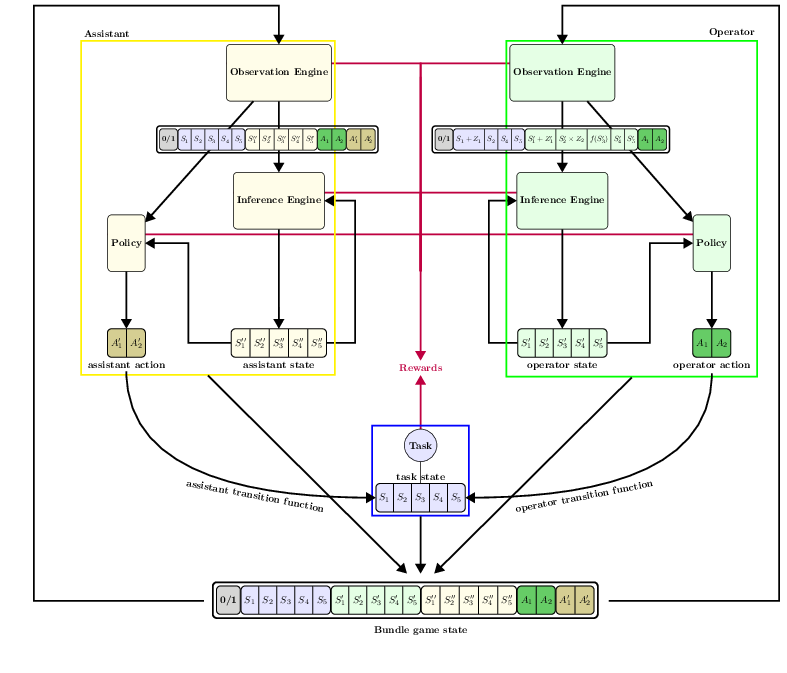
\includegraphics[height=\textheight]{fig/bundle.png} 
\end{frame}



\section{Library Components}

\begin{frame}{\textbf{Agents}}
\centering
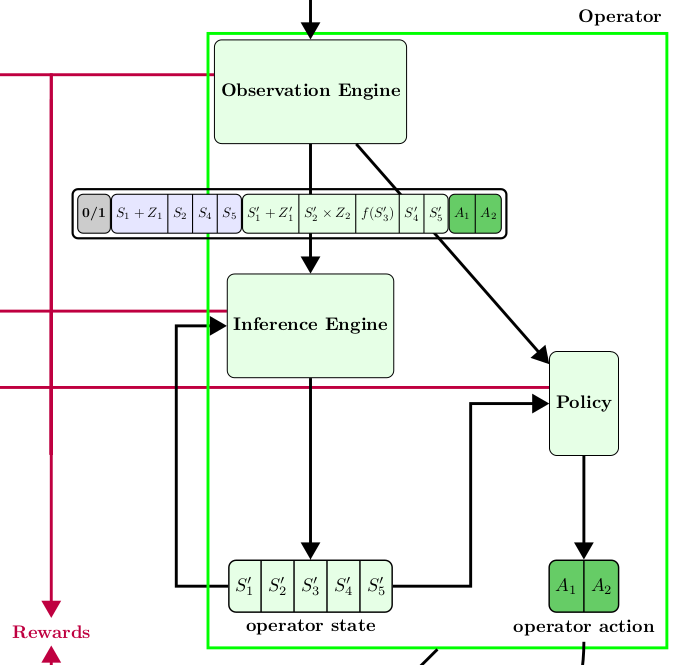
\includegraphics[height=.8\textheight]{fig/agents.png} 
\end{frame}

\begin{frame}[fragile]{\textbf{Creating an agent}}
\begin{adjustbox}{height=.4\textheight}\lstset{language=Python}
\lstset{frame=lines}
\lstset{label={lst:code_direct}}
\lstset{basicstyle=\footnotesize}
\begin{lstlisting}
class MyNewAgent(BaseAgent):
    """ Use this class as template to build your new agent.

    :param myparameter(type): explain the parameter here
    :return: what is returned
    :meta public:
    """
    def __init__(self, arg1, *args, **kwargs):
        self.arg1 = arg1


        agent_policy = kwargs.get('agent_policy')
        if agent_policy is None:
            # agent_policy =

        observation_engine = kwargs.get('observation_engine')
        if observation_engine is None:
            # observation_engine =

        inference_engine = kwargs.get('inference_engine')
        if inference_engine is None:
            # inference_engine =

        state = kwargs.get('state')
        if state is None:
            # state =

        super().__init__('user',
                            state = state,
                            policy = agent_policy,
                            observation_engine = observation_engine,
                            inference_engine = inference_engine
                            )

\end{lstlisting}
\end{adjustbox}
\end{frame}


\begin{frame}[fragile]{\textbf{States}}
States are first class objects:
\begin{itemize}
\item Filtering, flattening, clipping, casting, value checking and correcting properties
\item State Arithmetics possible (most Python users will work)
\item Iteration, Indexing possible
\end{itemize}

\begin{adjustbox}{width=.8\textwidth}
\lstset{language=Python}
\lstset{frame=lines}
\lstset{label={lst:code_direct}}
\lstset{basicstyle=\footnotesize}
\begin{lstlisting}
state = State()
state['Targets'] = StateElement(
            values = [numpy.array([0 for i in range(dimension)])],
            spaces = [gym.spaces.Box(-1,1, shape = (dimension,))],
            possible_values = [None],
            mode = 'warn'
        )
\end{lstlisting}
\end{adjustbox}

\end{frame}




\begin{frame}{\textbf{Observation Engine}}
\centering
\includegraphics[width=.8\textheight]{fig/observation_engine_general.pdf} 
\end{frame}

\begin{frame}[fragile]{\textbf{Creating an Observation Engine}}
\begin{adjustbox}{height=.4\textheight}\lstset{language=Python}
\lstset{frame=lines}
\lstset{label={lst:code_direct}}
\lstset{basicstyle=\footnotesize}
\begin{lstlisting}
class MyObservationEngine(BaseObservationEngine):
    def __init__(self, arg1, *args, **kwargs):
        super().__init__()
        self.type = 'enter type'
        self.arg1 = arg1

    def __content__(self):
        return _str

    def observe(self, game_state):
        game_state = copy.deepcopy(game_state)
        rewards = 0
        return game_state, rewards
\end{lstlisting}
\end{adjustbox}
\end{frame}

\begin{frame}{\textbf{Inference Engines}}
\centering
\includegraphics[height = .7\textheight]{fig/inference_engine.pdf} 
\end{frame}


\begin{frame}[fragile]{\textbf{Creating an Inference Engine}}
\begin{adjustbox}{height=.4\textheight}\lstset{language=Python}
\lstset{frame=lines}
\lstset{label={lst:code_direct}}
\lstset{basicstyle=\footnotesize}
\begin{lstlisting}
class MyInferenceEngine(BaseInferenceEngine):
    
    def __init__(self, arg1):
        super().__init__()
        self.arg1 = arg1


    def infer(self):
        """
        :return: (State) state, (float) reward

        :meta public:
        """
        observation = self.observation
        # alternatively:
        # observations = self.buffer
        if self.host.role == "user":
            state = observation['user_state']
        else:
            state = observation["assistant_state"]

        # do something with state

        return state, 0


    def render(self, *args, **kwargs):
       # display something
\end{lstlisting}
\end{adjustbox}
\end{frame}


\begin{frame}{\textbf{Policies}}
\centering
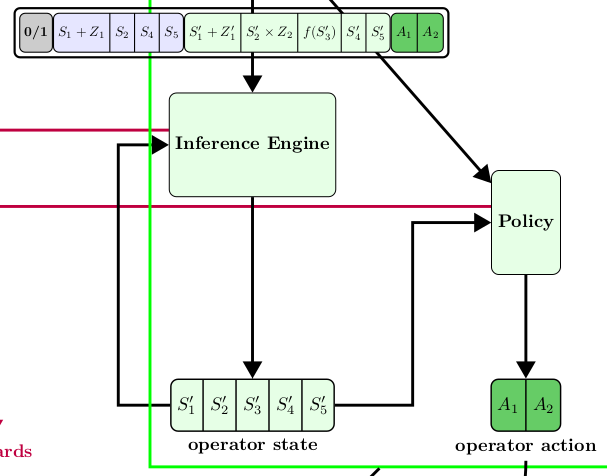
\includegraphics[height = .7\textheight]{fig/policy.png} 
\end{frame}

\begin{frame}[fragile]{\textbf{Creating a Policy}}
\begin{adjustbox}{height=.4\textheight}\lstset{language=Python}
\lstset{frame=lines}
\lstset{label={lst:code_direct}}
\lstset{basicstyle=\footnotesize}
\begin{lstlisting}
class MyNewPolicy(Policy):
 
    def __init__(self, arg1, *args, **kwargs):
        action_state =
        super().__init__(action_state, *args, **kwargs)
        self.arg1 = arg1
        

    def sample(self):
        action =
        reward = 
        return action, reward

    def reset(self):
        pass

\end{lstlisting}
\end{adjustbox}
\end{frame}


\begin{frame}{\textbf{Tasks}}
\centering
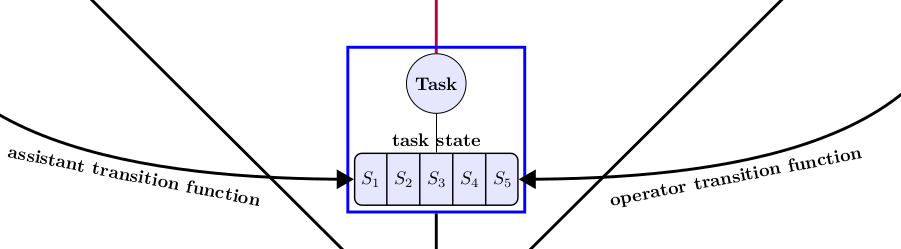
\includegraphics[width = \textwidth]{fig/tasks.png} 
\end{frame}

\begin{frame}[fragile]{\textbf{Creating a Task}}
\begin{adjustbox}{height=.4\textheight}\lstset{language=Python}
\lstset{frame=lines}
\lstset{label={lst:code_direct}}
\lstset{basicstyle=\footnotesize}
\begin{lstlisting}
class SimplePointingTask(InteractionTask):
 
    def __init__(self, arg1):
        super().__init__()
        self.arg1 = arg1

        self.state['mystate'] = StateElement(
                    values = None,
                    spaces = [gym.spaces.Discrete(2)],
                    possible_values = None,
                    mode = 'error'  )



    def reset(self, dic = None):
    
        super().reset()

        # set state to some value
        self.state['mystate'] =

        if dic is not None:
            super().reset(dic = dic)


    def user_step(self, *args, **kwargs):
   
        super().user_step()
        # do something

        return self.state, reward, is_done, {}


    def assistant_step(self, *args, **kwargs):
      
        super().assistant_step()
        # do something
        is_done = False
        return self.state, -1/2, is_done, {}

    def render(self,*args, mode="text"):
        # plot or print something

\end{lstlisting}
\end{adjustbox}
\end{frame}



\begin{frame}{\textbf{Bundles}}

\begin{minipage}{.3\textwidth}
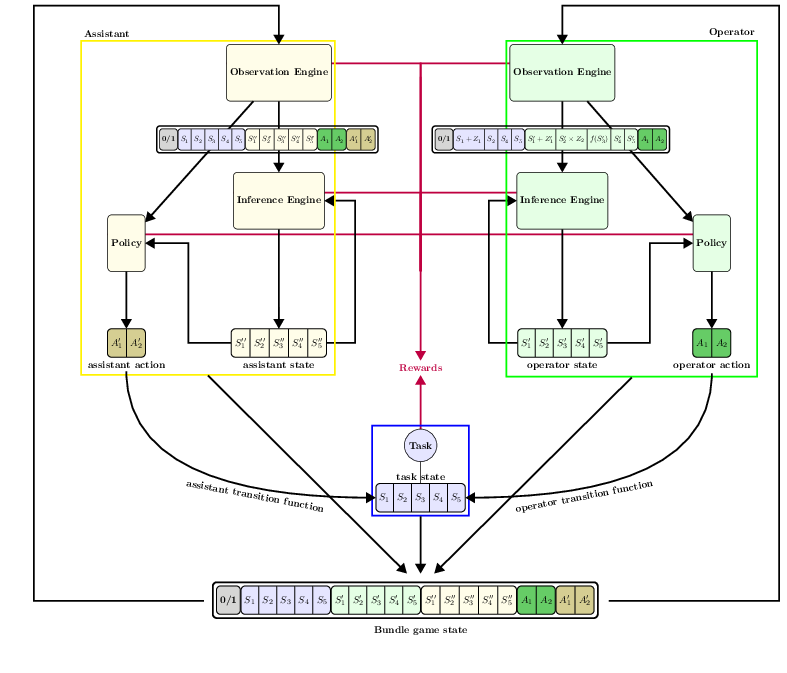
\includegraphics[width=\textwidth]{fig/bundle.png} 
\end{minipage}%
\begin{minipage}{.7\textwidth}
\begin{itemize}
\item Handles its own initialization procedure (e.g. allows dependent initialization of agents)
\item Handles the joint game state
\item Dispatches resets
\item Defines how one iteration should work (One can subclass the main Bundle class to redefine this)
\item Dispatches rendering
\end{itemize}
\end{minipage}
\end{frame}


\begin{frame}{\textbf{Bundles: A PlayUser Bundle}}
\centering
\includegraphics[height=.9\textheight]{fig/PlayUser.png} 
\end{frame}

\begin{frame}[fragile]{\textbf{Defining a Bundle}}
\begin{adjustbox}{width=\textwidth}\lstset{language=Python}
\lstset{frame=lines}
\lstset{label={lst:code_direct}}
\lstset{basicstyle=\footnotesize}
\begin{lstlisting}
class MyBundle(Bundle):
    def __init__(self, task, user, assistant, **kwargs):
        super().__init__(task, user, assistant, **kwargs)

    def reset(self, dic = {}):
        return super().reset(dic = dic)
		        
    def step(self, action):
      
        super().step(action)
		
        # Broadcast action if needed
		# have the users and assistant step
        # collect all rewards, check if task is done        
        return observation, rewards, is_done, sumrewards
        
        
\end{lstlisting}
\end{adjustbox}
\end{frame}



\begin{frame}{\textbf{List of Bundles}}

\resizebox{\textwidth}{!}{
\begin{tabulary}{.8\textwidth}{c c c c c c c }
\toprule 
  & Task & User & Assistant & User Action & Assistant Action & Comments \\ 
PlayUser & $\checkmark$ & $\checkmark$ & $\checkmark$ & Modeler & Policy & Evaluate user on-line \\ 
PlayAssistant & $\checkmark$ & $\checkmark$ & $\checkmark$ & Policy & Modeler & Evaluate assistant on-line \\ 
PlayNone & $\checkmark$ & $\checkmark$ & $\checkmark$ & Policy & Policy & Evaluate both off-line \\ 
PlayBoth & $\checkmark$ & $\checkmark$ & $\checkmark$ & Modeler & Modeler & Evaluate both on-line \\  
SinglePlayUser & $\checkmark$ &  & $\checkmark$ & Modeler & & Develop user models \\
SinglePlayUserAuto & $\checkmark$ &  & $\checkmark$ & Policy &  & Run user models \\
DevelopTask & $\checkmark$ &  &  & Modeler & Modeler & Helper to implement tasks \\
Train & --- & --- & --- & RL algorithm & RL algorithm & compatible with gym.Env\\
\bottomrule 
\end{tabulary} 
}
\end{frame}

\section{Some Examples and Use cases}

\begin{frame}{\textbf{Running example}}
\includegraphics[width=\textwidth, trim = {0 6cm 0 2cm}, clip]{fig/1.pdf} 
\begin{itemize}
\item User Goal:  Move the cursor (blue) to the goal target (green)
\item Assistant Goal: Help the user get there despite distractor targets (purple)
\item Modulation: cursor step = user action $\times$ assistant action
\item Careful Pointer: Indicates left ($-1$) or right ($+1$), sees everything except assistant state
\item Constant CD gain: Always outputs unit action, sees everything except user state (i.e. its goal)
\end{itemize}
\end{frame}


\begin{frame}[fragile]{\textbf{Running example -- Continued}}
\begin{adjustbox}{width=\textwidth}\lstset{language=Python}
\lstset{frame=lines}
\lstset{label={lst:code_direct}}
\lstset{basicstyle=\footnotesize}
\begin{lstlisting}
task = SimplePointingTask(gridsize = 31, number_of_targets = 8)
binary_user = CarefulPointer()
unitcdgain = ConstantCDGain(1)
bundle = PlayNone(task, binary_user, unitcdgain)
game_state = bundle.reset()
bundle.render('plotext')
while True:
    game_state, sum_rewards, is_done, rewards = bundle.step()
    bundle.render('plotext')
    if is_done:
        bundle.close()
        break
\end{lstlisting}
\end{adjustbox}
\end{frame}

\begin{frame}[fragile]{\textbf{Reinforcement Learning}}
Example: Training a user Model for a given assistant policy
\begin{adjustbox}{width=\textwidth}\lstset{language=Python}
\lstset{frame=lines}
\lstset{label={lst:code_direct}}
\lstset{basicstyle=\footnotesize}
\begin{lstlisting}
def make_env(rank, seed = 0):
        def _init():
            task = SimplePointingTask(gridsize = 31, number_of_targets = 8)
            unitcdgain = ConstantCDGain(1)

            policy = Policy(    action_space = [gym.spaces.Discrete(10)],
                                action_set = [-5 + i for i in range (5)] + [i+1 for i in range(5)],
                                action_values = None
            )

            user = CarefulPointer(agent_policy = policy)
            bundle = PlayUser(task, user, unitcdgain)

            observation_dict = OrderedDict({'task_state': OrderedDict({'Position': 0}),
             'user_state': OrderedDict({'Goal': 0})})
            
            env = Train(
                    bundle,
                    observation_mode = 'multidiscrete',
                    observation_dict = observation_dict
                    )
           env = ActionWrapper( env)

            env.seed(seed + rank)
            return env
        set_random_seed(seed)
        return _init
        
\end{lstlisting}
\end{adjustbox}
\end{frame}


\begin{frame}[fragile]{\textbf{RL -- continued}}
\begin{adjustbox}{width=\textwidth}
\lstset{language=Python}
\lstset{frame=lines}
\lstset{label={lst:code_direct}}
\lstset{basicstyle=\footnotesize}
\begin{lstlisting}
from stable_baselines3 import PPO
from stable_baselines3.common.vec_env import SubprocVecEnv
from stable_baselines3.common.env_util import make_vec_env
from stable_baselines3.common.utils import set_random_seed
        
if __name__ == '__main__':

    num_cpu = 3
    env = SubprocVecEnv([make_env(i) for i in range(num_cpu)])

    model = PPO('MlpPolicy', env, verbose=1)
    model.learn(total_timesteps=100000)
\end{lstlisting}
\end{adjustbox}
\end{frame}


\begin{frame}[fragile]{\textbf{Reusing trained model}}
Once trained, the model can be used as policy
\begin{adjustbox}{width=\textwidth}
\lstset{language=Python}
\lstset{frame=lines}
\lstset{label={lst:code_direct}}
\lstset{basicstyle=\footnotesize}
\begin{lstlisting}
class RLPolicy(BasePolicy):
   
    def __init__(self, *args, **kwargs):
        self.role = args[0]
        
        model_path = kwargs.get('model_path')
        learning_algorithm = kwargs.get('learning_algorithm')
        library = kwargs.get('library')
        self.training_env = kwargs.get('training_env')
        self.wrappers = kwargs.get('wrappers')
        
        # library checks and recover action state

        super().__init__(action_state, *args, **kwargs)

    def sample(self):
        nn_obs = self.training_env.unwrapped.convert_observation(self.observation)
        _action = self.model.predict(nn_obs)[0]
        for wrappers_name, (_cls, _args) in reversed(self.wrappers['actionwrappers'].items()):
            aw = _cls(self.training_env.unwrapped, *_args)
            _action = aw.action(_action)
        action = self.action_state['action']
        action['values'] = _action
        return action, 0
\end{lstlisting}
\end{adjustbox}
\end{frame}

\begin{frame}[fragile]{\textbf{Reusing trained model -- Continued}}
That policy can be plugged back in the agent
\begin{adjustbox}{width=.95\textwidth}
\lstset{language=Python}
\lstset{frame=lines}
\lstset{label={lst:code_direct}}
\lstset{basicstyle=\footnotesize}
\begin{lstlisting}
task = SimplePointingTask(gridsize = 31, number_of_targets = 8)
unitcdgain = ConstantCDGain(1)

# specifying user policy
action_wrappers = OrderedDict()
action_wrappers['ActionWrapper'] = (ActionWrapper, ())

policy = RLPolicy(
        'user',
        model_path =  'guide/models/basic_pointer_ppo',
        learning_algorithm = 'PPO',
        library = 'stable_baselines3',
        training_env = training_env,
        wrappers = {'actionwrappers': action_wrappers, 'observation_wrappers': {}}
          )
# Redefining the agent's policy 
user = CarefulPointer(agent_policy = policy)

bundle = PlayNone(task, user, unitcdgain)
game_state = bundle.reset()
bundle.render('plotext')

while True:
    observation, sum_reward, is_done, rewards = bundle.step()
    bundle.render('plotext')
    if is_done:
        break
\end{lstlisting}
\end{adjustbox}
\end{frame}

\begin{frame}{\textbf{Interaction technique: maximizing information gain}}

Assistant algorithm: find the next cursor position that is (on average) most informative to know which target is the user's goal

\begin{align*}
x^* = \max_x H(Y|X=x) - H(Y|\Theta, X=x)
\end{align*}

\begin{itemize}
\item $H = $ Shannon entropy
\item $Y = $ user action 
\item $X = $ cursor position
\item $p(\Theta = \theta)=$ prob. that target $\theta$ is user's goal
\end{itemize}
Bayesian updating scheme
\begin{itemize}
\item user action likelihood $p(Y=y | X=x, \Theta = \theta)$ $\longrightarrow$ feed a (synthetic) user policy to the assistant
\item maintain beliefs $p(\Theta = \theta | X=x, Y=y)$ $\longrightarrow$ Hold pmf in state + update via Inference engine
\end{itemize}

\end{frame}

\begin{frame}{\textbf{Maximizing information gain}}
\centering
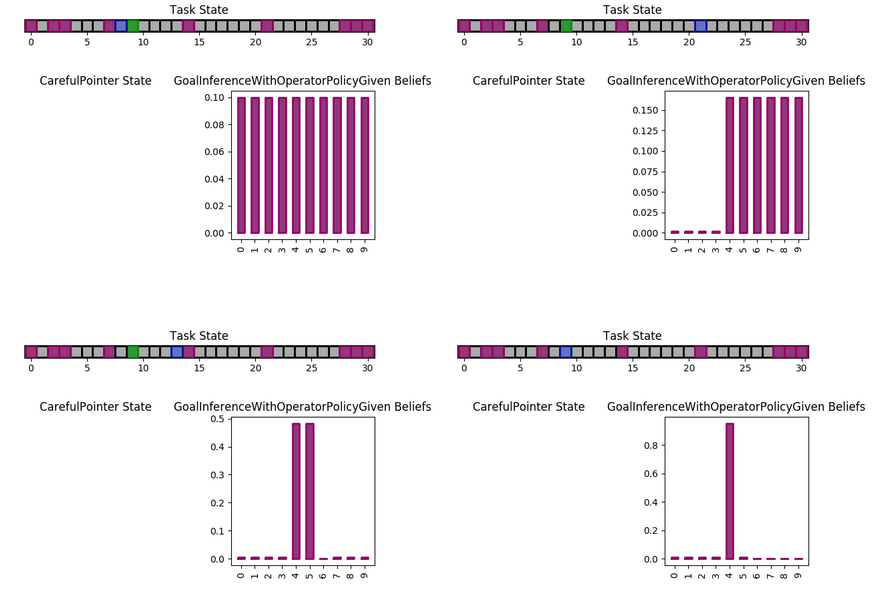
\includegraphics[width=\textwidth, height = .7\textheight, keepaspectratio]{fig/biggain.png} \\

Good performance, problem: cursor jumps around. We have to penalize cursor jumping.
\end{frame}


\begin{frame}{\textbf{Eye module}}
Adapted from Chen et al. 2021

\centering
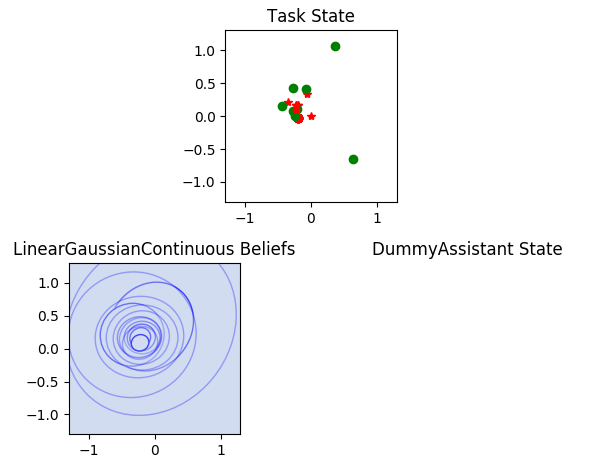
\includegraphics[width=.8\textwidth]{fig/eye.png} 
\end{frame}

\begin{frame}[fragile]{\textbf{Adding observation cost to cursor}}
Idea:
\begin{itemize}
\item We have a model that simulates the eye looking for a target.
\item When the cursor moves around at each step, we consider the old position of the cursor to be the start fixation and the new position of the cursor the target.
\item Use this somehow in an observation engine
\end{itemize}

First set up the pointing task as usual

\begin{adjustbox}{width=.95\textwidth}
\lstset{language=Python}
\lstset{frame=lines}
\lstset{label={lst:code_direct}}
\lstset{basicstyle=\footnotesize}
\begin{lstlisting}
pointing_task = OldPositionMemorizedSimplePointingTask(
	gridsize = 31, 
	number_of_targets = 8, 
	mode = 'position')
\end{lstlisting}
\end{adjustbox}
\end{frame}

\begin{frame}[fragile]{\textbf{Adding observation costs -- Continued}}
Now define the observation module


\begin{adjustbox}{width=.5\textwidth}
\lstset{language=Python}
\lstset{frame=lines}
\lstset{label={lst:code_direct}}
\lstset{basicstyle=\footnotesize}
\begin{lstlisting}
fitts_W = 4e-2
fitts_D = 0.8
perceptualnoise = 0.2
oculomotornoise = 0.2
task = ChenEyePointingTask(
	fitts_W, 
	fitts_D, 
	dimension = 1)
user = ChenEye( 
	perceptualnoise, 
	oculomotornoise, 
	dimension = 1)
	
obs_bundle = SinglePlayUserAuto(
	task, 
	user, 
	start_at_action = True)
\end{lstlisting}
\end{adjustbox}
\end{frame}

\begin{frame}[fragile]{\textbf{Wrapping it as an observation engine}}
Now wrap the bundle as an observation engine:
\begin{adjustbox}{width=.6\textwidth}
\lstset{language=Python}
\lstset{frame=lines}
\lstset{label={lst:code_direct}}
\lstset{basicstyle=\footnotesize}
\begin{lstlisting}
class ChenEyeObservationEngineWrapper(WrapAsObservationEngine):
    def __init__(self, obs_bundle):
        super().__init__(obs_bundle)

    def observe(self, game_state):
        # set observation bundle to the right state 
        # and cast it to the right space
        target = game_state['task_state']['Position'].cast(
        self.game_state['task_state']['Targets'])
        fixation = game_state['task_state']['OldPosition'].cast(
        self.game_state['task_state']['Fixation'])
        reset_dic = {'task_state':
                        {   'Targets': target,
                            'Fixation': fixation    }
                    }
        self.reset(dic = reset_dic)

        # perform the run
        is_done = False
        rewards = 0
        while True:
            obs, reward, is_done, _doc = self.step()
            rewards += reward
            if is_done:
                break
                
		# cast back to initial space and return
        obs['task_state'['Fixation'].cast(
        game_state['task_state']['OldPosition'])
        obs['task_state']['Targets'].cast(
        game_state['task_state']['Position'])

        return game_state, rewards

\end{lstlisting}
\end{adjustbox}
\end{frame}

\begin{frame}[fragile]{\textbf{Combining it with old observation engine}}
Combine it with old observation engine
\begin{adjustbox}{width=\textwidth}
\lstset{language=Python}
\lstset{frame=lines}
\lstset{label={lst:code_direct}}
\lstset{basicstyle=\footnotesize}
\begin{lstlisting}
# Define cascaded observation engine
cursor_tracker = ChenEyeObservationEngineWrapper(obs_bundle)
default_observation_engine = RuleObservationEngine(
       base_user_engine_specification,
            )
cascaded_observation_engine = CascadedObservationEngine(
[cursor_tracker, default_observation_engine])

\end{lstlisting}
\end{adjustbox}
and plug it in the old user, to have  new observation engine
\begin{adjustbox}{width=\textwidth}
\lstset{language=Python}
\lstset{frame=lines}
\lstset{label={lst:code_direct}}
\lstset{basicstyle=\footnotesize}
\begin{lstlisting}
binary_user = CarefulPointer(
	observation_engine = cascaded_observation_engine)
    BIGpointer = BIGGain()
    bundle = PlayAssistant(pointing_task, binary_user, BIGpointer)


\end{lstlisting}
\end{adjustbox}

\vspace{\baselineskip}

rewards:
[[-1, 0, 0, -0.5, 0, 0, 0, -0.5], [-13, 0, 0, -0.5, 0, 0, 0, -0.5], [-2, 0, 0, -0.5, 0, 0, 0, -0.5]]

\end{frame}


\begin{frame}{\textbf{Example with Complex Policy and Observation Engine}}
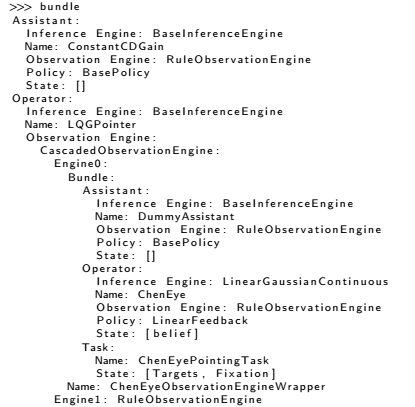
\includegraphics[width=.49\textwidth]{fig/b_1.png}%
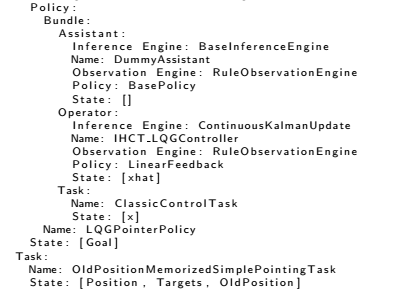
\includegraphics[width=.49\textwidth]{fig/b_2.png}
\end{frame}

\begin{frame}{\textbf{What's next}}
\begin{itemize}
\item Essentially making the code more consistent and easier to use for an end-user
\item Get an idea of performance
\item Make bundles to help construct models (e.g. parameter inference and recovery checks)
\item Interface with real tasks and other languages
\end{itemize}
\end{frame}


\begin{frame}{\textbf{What's next?}}
\centering%
\resizebox{\textwidth}{!}{
\begin{tabular}{lcccccc}
    & & \textbf{Working now} & \textbf{Step 1} & \textbf{Step 2} & \textbf{Step 3} & \textbf{Final Setup}  \\
    \toprule
    \multirow{2}{*}{\textbf{Evaluation}}& Synthetic User Model & \checkmark & \checkmark & \checkmark &  & \checkmark \\
    & Real User &  &  & & \checkmark & \checkmark  \\
    \cmidrule{2-7}
    \multirow{2}{*}{\textbf{Task}}& Abstract Task & \checkmark & \checkmark & \checkmark & & \checkmark\\
    & Realistic Task &  & & & \checkmark &  \checkmark \\
    \cmidrule{2-7}
    \multirow{4}{*}{\textbf{Assistance}}& User Agnostic  & \checkmark & \checkmark & \checkmark & \checkmark & \checkmark \\
    & User Model Given & \checkmark & \checkmark & \checkmark & \checkmark & \checkmark \\ & User Model Structure Given, parameters learned &  & \checkmark & \checkmark & \checkmark & \checkmark \\ & User-gnostic, nothing given & & \checkmark & \checkmark  & \checkmark & \checkmark \\
    \cmidrule{2-7}
   	 \multirow{3}{*}{\textbf{User Model}}& Explicit likelihood-based model & \checkmark & \checkmark & \checkmark &  --- &  \checkmark \\
    & trained/tuned user model & \checkmark & \checkmark & \checkmark & --- &  \checkmark \\ & Nested simulation models & \checkmark & \checkmark & \checkmark & --- &  \checkmark \\
    \cmidrule{2-7}
     \multirow{2}{*}{\textbf{Adaptivity}}& Static policies & \checkmark & \checkmark & & & \checkmark \\
     & Adaptive Assistance with adaptive user policy &  & & \checkmark & \checkmark & \checkmark \\
    \bottomrule
\end{tabular}
}
\end{frame}
\end{document}